\documentclass{standalone}
\usepackage{tikz}
\usetikzlibrary{patterns, positioning}
\usepackage[sfdefault]{ClearSans} %% option 'sfdefault' activates Clear Sans as the default text font
\usepackage[T1]{fontenc}

\begin{document}
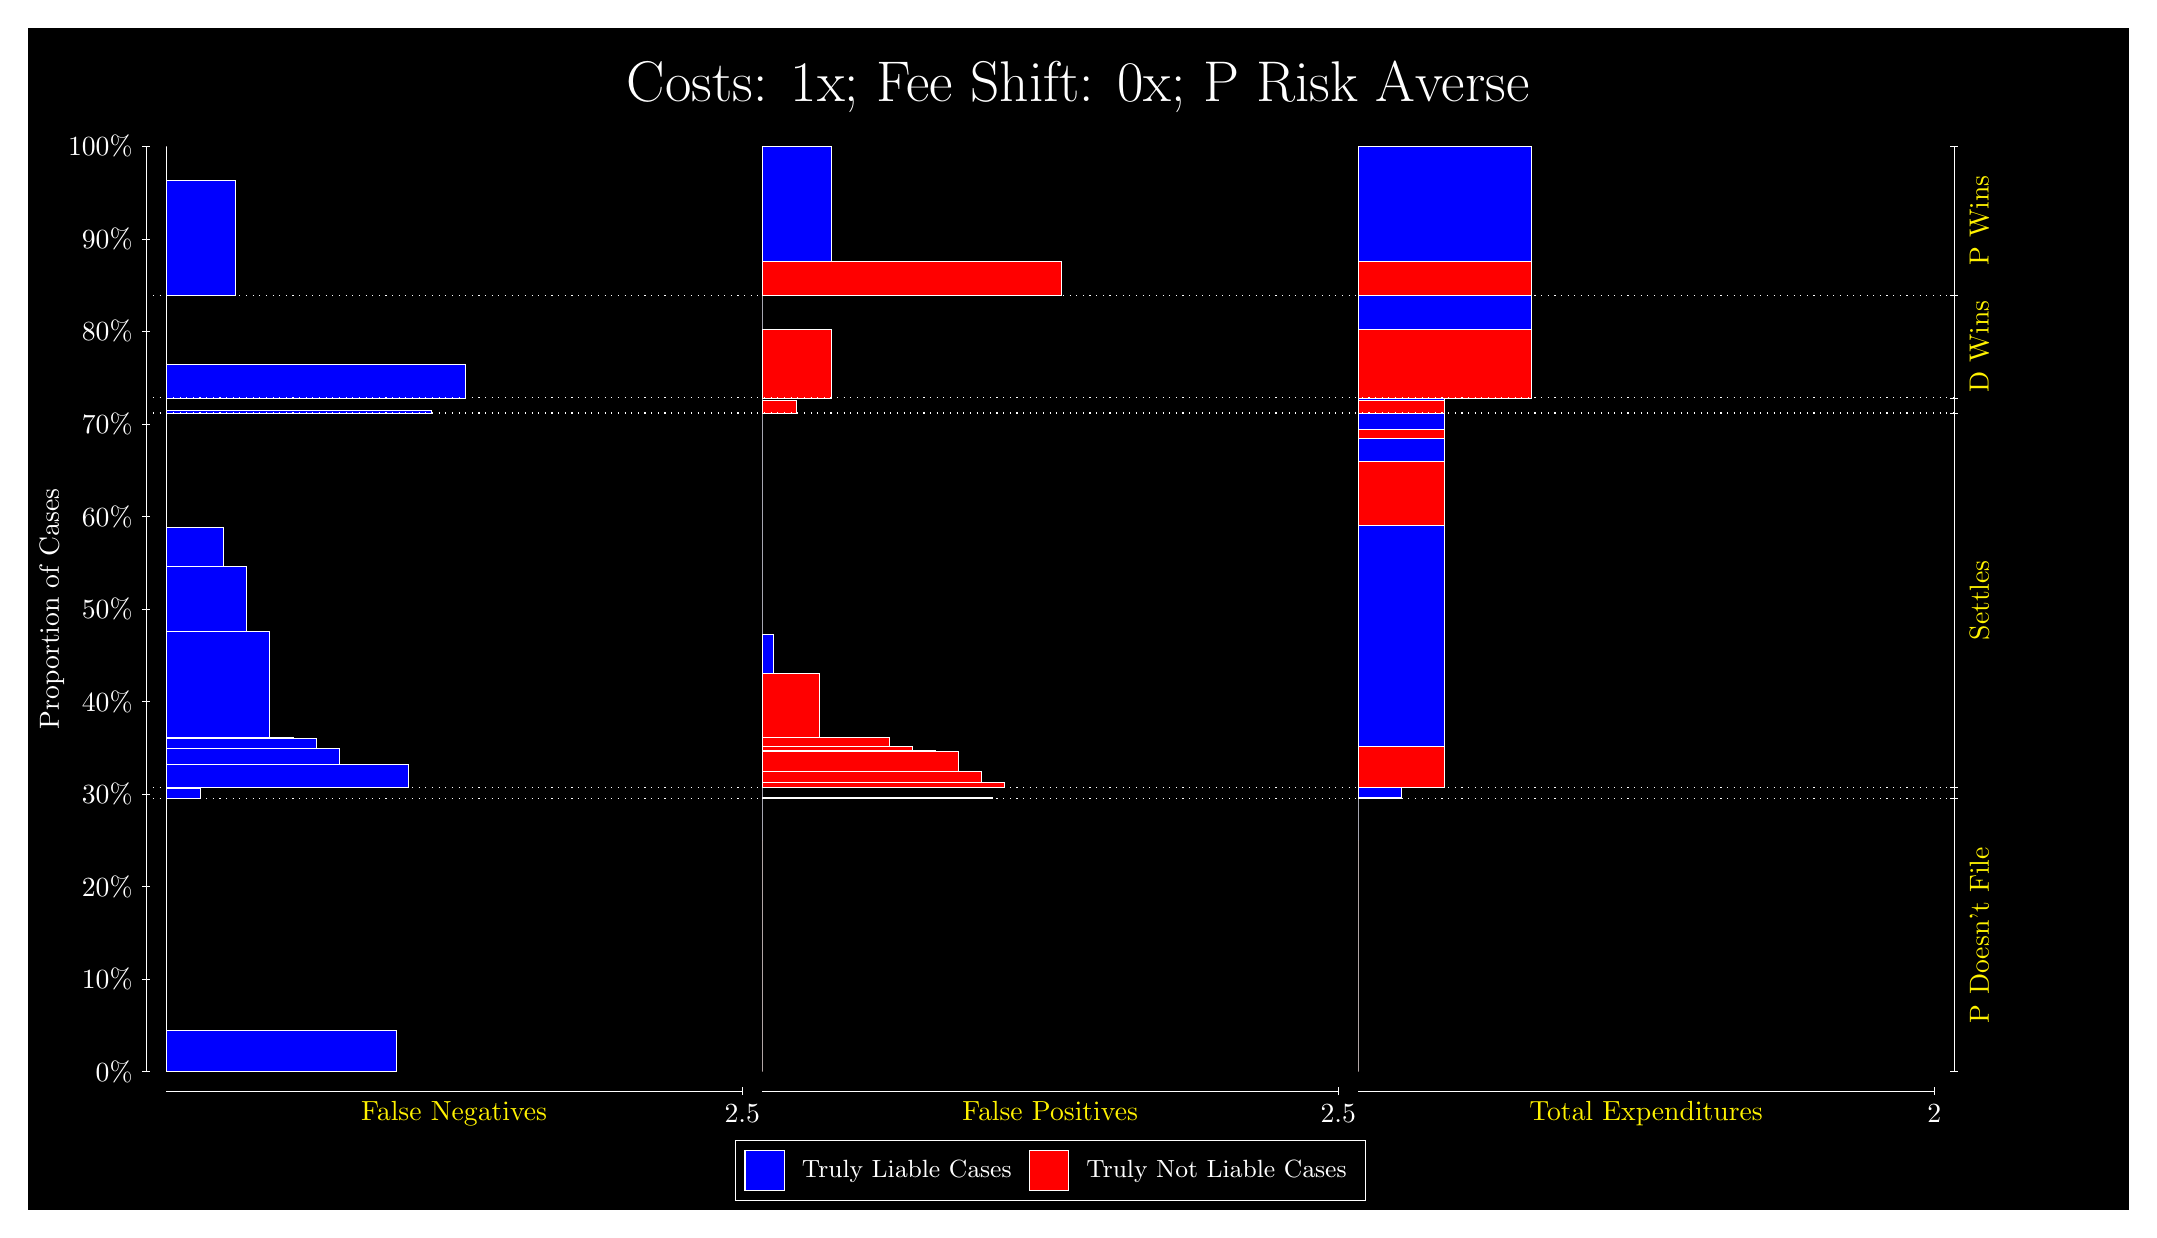
\begin{tikzpicture}
\draw[fill=black] (0,0) rectangle (26.667,15);
\draw[text=white] (0,13.5) rectangle (26.667,15) node[midway] {\huge Costs: 1x; Fee Shift: 0x; P Risk Averse};
\draw[white, very thin] (1.5,1.75) -- (1.5,13.5);
\node[rotate=90, text=white, anchor=center] at (0.3, 7.625) {Proportion of Cases};
\draw[white, very thin] (1.45,1.75) -- (1.55,1.75);
\node[text=white, anchor=east] at (1.45, 1.75) {0\%};
\draw[white, very thin] (1.45,2.925) -- (1.55,2.925);
\node[text=white, anchor=east] at (1.45, 2.925) {10\%};
\draw[white, very thin] (1.45,4.1) -- (1.55,4.1);
\node[text=white, anchor=east] at (1.45, 4.1) {20\%};
\draw[white, very thin] (1.45,5.275) -- (1.55,5.275);
\node[text=white, anchor=east] at (1.45, 5.275) {30\%};
\draw[white, very thin] (1.45,6.45) -- (1.55,6.45);
\node[text=white, anchor=east] at (1.45, 6.45) {40\%};
\draw[white, very thin] (1.45,7.625) -- (1.55,7.625);
\node[text=white, anchor=east] at (1.45, 7.625) {50\%};
\draw[white, very thin] (1.45,8.8) -- (1.55,8.8);
\node[text=white, anchor=east] at (1.45, 8.8) {60\%};
\draw[white, very thin] (1.45,9.975) -- (1.55,9.975);
\node[text=white, anchor=east] at (1.45, 9.975) {70\%};
\draw[white, very thin] (1.45,11.15) -- (1.55,11.15);
\node[text=white, anchor=east] at (1.45, 11.15) {80\%};
\draw[white, very thin] (1.45,12.325) -- (1.55,12.325);
\node[text=white, anchor=east] at (1.45, 12.325) {90\%};
\draw[white, very thin] (1.45,13.5) -- (1.55,13.5);
\node[text=white, anchor=east] at (1.45, 13.5) {100\%};

\draw[white, very thin] (24.457,1.75) -- (24.457,13.5);
\draw[white, very thin] (24.407,1.75) -- (24.507,1.75);
\node[anchor=west] at (24.407, 1.75) {};
\draw[white, very thin] (24.407,5.2153) -- (24.507,5.2153);
\node[anchor=west] at (24.407, 5.2153) {};
\draw[white, very thin] (24.407,5.3566) -- (24.507,5.3566);
\node[anchor=west] at (24.407, 5.3566) {};
\draw[white, very thin] (24.407,10.113) -- (24.507,10.113);
\node[anchor=west] at (24.407, 10.113) {};
\draw[white, very thin] (24.407,10.305) -- (24.507,10.305);
\node[anchor=west] at (24.407, 10.305) {};
\draw[white, very thin] (24.407,11.609) -- (24.507,11.609);
\node[anchor=west] at (24.407, 11.609) {};
\draw[white, very thin] (24.407,13.5) -- (24.507,13.5);
\node[anchor=west] at (24.407, 13.5) {};

\draw[white, very thin, fill=blue] (1.75,1.75) rectangle (4.6775,2.2751);
\draw[white, very thin, fill=red] (1.75,2.2751) rectangle (1.75,5.2153);
\draw[white, very thin, fill=blue] (1.75,5.2153) rectangle (2.1891,5.3428);
\draw[white, very thin, fill=red] (1.75,5.3428) rectangle (1.75,5.3566);
\draw[white, very thin, fill=blue] (1.75,5.3566) rectangle (4.8239,5.6477);
\draw[white, very thin, fill=blue] (1.75,5.6477) rectangle (3.9457,5.8568);
\draw[white, very thin, fill=blue] (1.75,5.8568) rectangle (3.6529,5.9836);
\draw[white, very thin, fill=blue] (1.75,5.9836) rectangle (3.3602,5.9948);
\draw[white, very thin, fill=blue] (1.75,5.9948) rectangle (3.0674,7.3359);
\draw[white, very thin, fill=blue] (1.75,7.3359) rectangle (2.7746,8.1633);
\draw[white, very thin, fill=blue] (1.75,8.1633) rectangle (2.4819,8.6559);
\draw[white, very thin, fill=red] (1.75,8.6559) rectangle (1.75,10.113);
\draw[white, very thin, fill=blue] (1.75,10.113) rectangle (5.1167,10.148);
\draw[white, very thin, fill=red] (1.75,10.148) rectangle (1.75,10.305);
\draw[white, very thin, fill=blue] (1.75,10.305) rectangle (5.5558,10.732);
\draw[white, very thin, fill=red] (1.75,10.732) rectangle (1.75,11.609);
\draw[white, very thin, fill=blue] (1.75,11.609) rectangle (2.6283,13.07);
\draw[white, very thin, fill=red] (1.75,13.07) rectangle (1.75,13.5);
\draw[white, very thin, fill=red] (9.3189,1.75) rectangle (9.3189,4.6902);
\draw[white, very thin, fill=blue] (9.3189,4.6902) rectangle (9.3189,5.2153);
\draw[white, very thin, fill=red] (9.3189,5.2153) rectangle (12.246,5.2292);
\draw[white, very thin, fill=blue] (9.3189,5.2292) rectangle (9.3189,5.3566);
\draw[white, very thin, fill=red] (9.3189,5.3566) rectangle (12.393,5.4248);
\draw[white, very thin, fill=red] (9.3189,5.4248) rectangle (12.1,5.5571);
\draw[white, very thin, fill=red] (9.3189,5.5571) rectangle (11.807,5.8137);
\draw[white, very thin, fill=red] (9.3189,5.8137) rectangle (11.515,5.8252);
\draw[white, very thin, fill=red] (9.3189,5.8252) rectangle (11.222,5.8848);
\draw[white, very thin, fill=red] (9.3189,5.8848) rectangle (10.929,6.0011);
\draw[white, very thin, fill=red] (9.3189,6.0011) rectangle (10.051,6.8135);
\draw[white, very thin, fill=blue] (9.3189,6.8135) rectangle (9.4652,7.3061);
\draw[white, very thin, fill=blue] (9.3189,7.3061) rectangle (9.3189,10.113);
\draw[white, very thin, fill=red] (9.3189,10.113) rectangle (9.758,10.269);
\draw[white, very thin, fill=blue] (9.3189,10.269) rectangle (9.3189,10.305);
\draw[white, very thin, fill=red] (9.3189,10.305) rectangle (10.197,11.182);
\draw[white, very thin, fill=blue] (9.3189,11.182) rectangle (9.3189,11.609);
\draw[white, very thin, fill=red] (9.3189,11.609) rectangle (13.125,12.04);
\draw[white, very thin, fill=blue] (9.3189,12.04) rectangle (10.197,13.5);
\draw[white, very thin, fill=red] (16.888,1.75) rectangle (16.888,4.6902);
\draw[white, very thin, fill=blue] (16.888,4.6902) rectangle (16.888,5.2153);
\draw[white, very thin, fill=red] (16.888,5.2153) rectangle (17.437,5.2292);
\draw[white, very thin, fill=blue] (16.888,5.2292) rectangle (17.437,5.3566);
\draw[white, very thin, fill=red] (16.888,5.3566) rectangle (17.986,5.8848);
\draw[white, very thin, fill=blue] (16.888,5.8848) rectangle (17.986,8.6839);
\draw[white, very thin, fill=red] (16.888,8.6839) rectangle (17.986,9.4963);
\draw[white, very thin, fill=blue] (16.888,9.4963) rectangle (17.986,9.7874);
\draw[white, very thin, fill=red] (16.888,9.7874) rectangle (17.986,9.9037);
\draw[white, very thin, fill=blue] (16.888,9.9037) rectangle (17.986,10.113);
\draw[white, very thin, fill=red] (16.888,10.113) rectangle (17.986,10.269);
\draw[white, very thin, fill=blue] (16.888,10.269) rectangle (17.986,10.305);
\draw[white, very thin, fill=red] (16.888,10.305) rectangle (19.083,11.182);
\draw[white, very thin, fill=blue] (16.888,11.182) rectangle (19.083,11.609);
\draw[white, very thin, fill=red] (16.888,11.609) rectangle (19.083,12.04);
\draw[white, very thin, fill=blue] (16.888,12.04) rectangle (19.083,13.5);
\draw[white, dotted] (1.5,5.2153) -- (24.457,5.2153);
\draw[white, dotted] (1.5,5.3566) -- (24.457,5.3566);
\draw[white, dotted] (1.5,10.113) -- (24.457,10.113);
\draw[white, dotted] (1.5,10.305) -- (24.457,10.305);
\draw[white, dotted] (1.5,11.609) -- (24.457,11.609);
\draw[white, very thin] (1.75,1.5) -- (9.0689,1.5);
\node[text=yellow, anchor=north] at (5.4094, 1.5) {False Negatives};
\draw[white, very thin] (9.0689,1.45) -- (9.0689,1.55);
\node[text=white, anchor=north] at (9.0689, 1.45) {2.5};

\draw[white, very thin] (9.3189,1.5) -- (16.638,1.5);
\node[text=yellow, anchor=north] at (12.978, 1.5) {False Positives};
\draw[white, very thin] (16.638,1.45) -- (16.638,1.55);
\node[text=white, anchor=north] at (16.638, 1.45) {2.5};

\draw[white, very thin] (16.888,1.5) -- (24.207,1.5);
\node[text=yellow, anchor=north] at (20.547, 1.5) {Total Expenditures};
\draw[white, very thin] (24.207,1.45) -- (24.207,1.55);
\node[text=white, anchor=north] at (24.207, 1.45) {2};

\node[text=yellow, centered, rotate=90] at (24.777, 3.4827) {P Doesn't File};

\node[text=yellow, centered, rotate=90] at (24.777, 7.7347) {Settles};

\node[text=yellow, centered, rotate=90] at (24.777, 10.957) {D Wins};
\node[text=yellow, centered, rotate=90] at (24.777, 12.555) {P Wins};

\draw (12.978300999999998,1.5) node[draw=none] (baseCoordinate) {};
\begin{scope}[align=center]
        \matrix[scale=0.5, draw=white, below=0.5cm of baseCoordinate, nodes={draw}, column sep=0.1cm]{
            \node[rectangle, draw, minimum width=0.5cm, minimum height=0.5cm, fill=blue] {}; &
            \node[draw=none, font=\small, text=white] (B) {Truly Liable Cases}; &
            \node[rectangle, draw, minimum width=0.5cm, minimum height=0.5cm, fill=red] {}; &
            \node[draw=none, font=\small, text=white] (B) {Truly Not Liable Cases}; \\
            };
\end{scope}

\end{tikzpicture}
\end{document}